%!TEX program = xelatex

% ==================== 模板与文档开始 ====================
% 加载厦门大学研究生论文模板，统一设置论文的版式、字体和格式。
\documentclass{xmu-graduate}
% 文档开始；下面先填写封面、声明和答辩委员会所需的信息。
\begin{document}

% ==================== 封面与声明类型 ====================
% 演示数据；实际提交前按学院要求选择封面并填写真实信息。
% 封面类型：degree 为学位论文，practice 为实践成果总结报告。
\thesiscover{degree} % degree 或 practice，必须显式选择
% 人工智能使用声明类型：used 表示使用过，unused 表示未使用。
\aideclaration{used} % used 或 unused，必须显式选择

% ==================== 论文题目与作者信息 ====================
% 论文题目：两个花括号依次填写中文题目和英文题目。
\title{集成电路工程研究示例}{A Sample Study in Integrated Circuit Engineering}
% 作者姓名。
\author{示例作者}
% 作者学号。
\idn{123456789}

% ==================== 学位与专业信息 ====================
% 学位层次，如硕士、博士。
\degreelevel{硕士}
% 学位类型，如学术学位、专业学位；用于 degree 类型封面。
\degreetype{专业学位}
% 专业名称。
\subject{集成电路工程}

% ==================== 导师信息 ====================
% 指导教师姓名；用于 degree 类型封面。
\advisor{示例教授}
% 校内导师姓名；用于 practice 类型封面。
\campusadvisor{示例教授}
% 行业导师姓名；用于 practice 类型封面。
\industryadvisor{示例高级工程师}

% ==================== 日期信息 ====================
% 论文答辩日期。
\defensedate{2026年10月}
% 学位授予日期。
\awarddate{2026年12月}
% 封面底部显示的日期。
\coverdate{2026年10月}

% ==================== 中英文关键词 ====================
% 关键词：两个花括号依次填写中文关键词和英文关键词。
\keywords{集成电路；芯片设计；验证}{Integrated Circuits; Chip Design; Verification}

% ==================== 原创性声明信息 ====================
% 声明中的三个括号：填写实际内容；空值将划去占位区域。
% 原创性声明中的课题（组）信息，对应第一个括号。
\researchproject{}
% 原创性声明中的经费或实验室资助信息，对应第二个括号。
\researchfunding{}
% 完成研究的实验室名称，对应第三个括号。
\researchlab{}

% ==================== 人工智能工具使用信息 ====================
% 仅选择 used 时按实际情况填写。
% 使用的生成式人工智能工具名称。
\aitools{}
% 人工智能工具的具体用途。
\aiusage{}

% ==================== 答辩委员会信息 ====================
% 答辩委员会主席：依次填写姓名、职称和单位。
\committeechair{示例姓名}{教授}{示例大学}
% 答辩委员会委员：每行一位，依次填写姓名、职称和单位。
\committeemember{示例委员甲}{教授}{示例研究院}
% 答辩委员会委员：每行一位，依次填写姓名、职称和单位。
\committeemember{示例委员乙}{副教授}{示例大学}

% ==================== 生成封面 ====================
% 根据上方填写的信息生成封面。
\maketitle

% ==================== 生成原创性声明 ====================
% 生成原创性声明页。
\makeoriginality

% ==================== 生成著作权使用声明 ====================
% 生成著作权使用声明页。
\makecopyright

% ==================== 生成人工智能工具声明 ====================
% 根据 used 或 unused 的设置生成相应的人工智能工具声明页。
\makeaideclaration

% ==================== 中文摘要 ====================
% 中文摘要：在此环境内撰写摘要正文，关键词由上方 keywords 命令设置。
\begin{abstract}
本示例展示研究生论文的结构和格式。正式论文应按学校要求撰写约六百字中文摘要，并按实际研究内容填写关键词。
\end{abstract}

% ==================== 英文摘要 ====================
% 英文摘要：在此环境内撰写英文摘要正文。
\begin{enabstract}
This sample demonstrates the structure and formatting of a graduate thesis. Replace this text with the actual abstract and keywords before submission.
\end{enabstract}

% ==================== 目录 ====================
% 自动生成目录，目录条目来自正文中的章、节标题。
\tableofcontents

% ==================== 论文正文 ====================
% 载入两个示例章节；具体章节内容在对应文件中编写。
% 本文件由 main.tex 载入，无需重复声明文档类或 document 环境。
\xmuchapter{研究背景与基础排版示例}{Research Background and Basic Typesetting}
\label{chap:sample-background}

\xmusection{研究背景与目标}{Research Background and Objectives}
\label{sec:sample-objectives}

本章演示正文、各级标题、图片、三线表、文献引用和数学公式的基本写法。
全文以输入与输出之间的线性关系为说明对象，所有模型和数据均为排版示例，
不代表实际研究结论。关于 \TeX{} 排版系统的基础知识，可参阅相关文献\cite{samplebook}。
正文中的补充说明可以使用脚注\footnote{示例注释：脚注适合放置补充解释，不宜替代正文中的关键论述。}。

\xmusubsection{研究问题}{Research Problem}

设输入量为 $x$，输出量为 $y$，研究目标是利用观测样本估计二者之间的关系。
正文中可以使用\textbf{加粗文字}强调重要概念，也可以用\emph{强调文字}标记术语。
符号、变量和简短表达式使用行内公式，例如 $x \in \mathbb{R}$ 和 $y = ax + b$。

% 更细一级的标题使用标准命令；模板目录默认只显示到 subsection。
\subsubsection{基本假设}

为便于说明，作如下假设：
\begin{enumerate}
    \item 输入量和输出量均为标量，且在相同条件下采集。
    \item 输入与输出之间近似满足线性关系。
    \item 测量误差以加性噪声的形式影响观测结果。
\end{enumerate}

\xmusubsection{研究内容}{Research Scope}

本示例主要包含以下内容：
\begin{itemize}
    \item 建立输入与输出之间的数学模型，说明符号的含义。
    \item 通过图片和表格展示研究对象与参数设置。
    \item 在第\ref{chap:sample-results}章中给出估计方法和结果分析。
\end{itemize}

\xmusection{图片与表格示例}{Figures and Tables}

图片放置于项目的 figures 文件夹，通过已有的图形路径设置即可直接按文件名载入。
图\ref{fig:sample}使用项目已有的校名图片，演示图片居中、按正文宽度缩放、
图题、标签和资料来源的写法；正式论文中应替换为与研究内容相关的图片。

\begin{figure}[htbp]
    \centering
    \includegraphics[width=0.55\textwidth]{xmu-logo-text.jpg}
    \caption{图片插入与图题排版示例}
    \label{fig:sample}
    \floatnote{资料来源：项目已有的厦门大学校名图片，仅用于演示图片排版。}
\end{figure}

表\ref{tab:sample}给出示例模型采用的参数。表题放在表格上方，
表头使用模板提供的加粗命令，表格下方单独标注资料来源。

\begin{table}[htbp]
    \centering
    \caption{示例模型参数设置}
    \label{tab:sample}
    \floatunit{单位：无量纲}
    \begin{tabular}{lcl}
        \toprule
        \tablehead{参数} & \tablehead{取值} & \tablehead{说明} \\
        \midrule
        $a$ & 2.0 & 线性模型斜率 \\
        $b$ & 1.0 & 线性模型截距 \\
        $N$ & 5 & 观测样本数量 \\
        \bottomrule
    \end{tabular}
    \floatnote{资料来源：作者构造的示例参数，仅用于排版演示。}
\end{table}

\xmusection{数学公式与交叉引用}{Equations and Cross-References}

考虑测量误差后，第 $i$ 个样本的观测模型可写为
\begin{equation}
    y_i = a x_i + b + \varepsilon_i, \qquad i = 1,2,\ldots,N,
    \label{eq:sample-model}
\end{equation}
其中，$a$ 为斜率，$b$ 为截距，$\varepsilon_i$ 为测量误差，$N$ 为样本数量。
式\eqref{eq:sample-model}的编号由模板自动生成。

将各个样本按行排列，可将式\eqref{eq:sample-model}写为矩阵形式：
\begin{align}
    \mathbf{y} &= \mathbf{X}\boldsymbol{\theta} + \boldsymbol{\varepsilon},
    \label{eq:sample-matrix} \\
    \mathbf{X} &=
    \begin{bmatrix}
        x_1 & 1 \\
        x_2 & 1 \\
        \vdots & \vdots \\
        x_N & 1
    \end{bmatrix},
    \qquad
    \boldsymbol{\theta} =
    \begin{bmatrix}
        a \\
        b
    \end{bmatrix}.
    \label{eq:sample-design}
\end{align}
其中，$\mathbf{y} = [y_1,\ldots,y_N]^{\mathrm{T}}$，
$\boldsymbol{\varepsilon} = [\varepsilon_1,\ldots,\varepsilon_N]^{\mathrm{T}}$。
第\ref{chap:sample-results}章将依据式\eqref{eq:sample-matrix}估计模型参数。

\xmusection{本章小结}{Chapter Summary}

本章展示了常用的标题层次、段落、列表、脚注、文献引用、图片、三线表和公式。
图\ref{fig:sample}、表\ref{tab:sample}以及式\eqref{eq:sample-model}
分别演示了图片、表格和公式的交叉引用。下一章进一步展示方法描述和结果分析的排版。

% 本文件接续 sample_chapter_1.tex；各章的图、表和公式标签应保持唯一。
\xmuchapter{研究方法与结果排版示例}{Research Methods and Result Presentation}
\label{chap:sample-results}

\xmusection{参数估计方法}{Parameter Estimation Method}

本章以第\ref{chap:sample-background}章的线性模型为例，
演示方法说明、多行公式、分段函数、结果曲线、数据表格和算法的排版。
全部数值均为人为构造的示例数据\footnote{本章数据仅用于检查图表和公式的显示效果，不能作为实验结果使用。}。
文献引用沿用项目现有的参考文献条目，关于排版系统的介绍可参阅文献\cite{samplebook}。

\xmusubsection{最小二乘估计}{Least-Squares Estimation}

对于式\eqref{eq:sample-model}，定义预测值为 $\hat{y}_i = \hat{a}x_i + \hat{b}$。
通过最小化观测值与预测值之间的平方误差，可得到参数估计：
\begin{align}
    J(a,b) &= \sum_{i=1}^{N}\left[y_i-(ax_i+b)\right]^2,
    \label{eq:sample-objective} \\
    \hat{\boldsymbol{\theta}} &=
    \underset{\boldsymbol{\theta}}{\operatorname{arg\,min}}\,
    \left\|\mathbf{y}-\mathbf{X}\boldsymbol{\theta}\right\|_2^2.
    \label{eq:sample-estimate}
\end{align}
当式\eqref{eq:sample-design}中的矩阵 $\mathbf{X}$ 列满秩时，估计结果可写为
\begin{equation}
    \hat{\boldsymbol{\theta}} =
    \left(\mathbf{X}^{\mathrm{T}}\mathbf{X}\right)^{-1}
    \mathbf{X}^{\mathrm{T}}\mathbf{y}.
    \label{eq:sample-solution}
\end{equation}

\xmusubsection{评价指标与分段函数}{Evaluation Metrics and Piecewise Function}

以均方根误差衡量预测结果与观测结果的差异：
\begin{equation}
    E_{\mathrm{RMSE}} =
    \sqrt{\frac{1}{N}\sum_{i=1}^{N}\left(y_i-\hat{y}_i\right)^2}.
    \label{eq:sample-rmse}
\end{equation}
为演示分段函数，设定误差阈值 $\tau = 0.15$，并定义示例判定函数
\begin{equation}
    q(E) =
    \begin{cases}
        1, & 0 \leq E \leq \tau, \\
        0, & E > \tau.
    \end{cases}
    \label{eq:sample-criterion}
\end{equation}
其中，$q(E)=1$ 表示误差满足示例阈值。该阈值仅用于说明公式写法。

\xmusection{示例数据与结果分析}{Sample Data and Result Analysis}

\xmusubsection{数据表格}{Data Table}

取表\ref{tab:sample}中的参数，令输入量依次为 $0$、$1$、$2$、$3$ 和 $4$，
构造表\ref{tab:sample-results}中的观测数据。对应的估计参数为
$\hat{a}=2.0$、$\hat{b}=1.0$。

\begin{table}[htbp]
    \centering
    \caption{观测值、预测值与误差对比}
    \label{tab:sample-results}
    \floatunit{单位：无量纲}
    \begin{tabular}{ccccc}
        \toprule
        \tablehead{样本序号} & \tablehead{输入值 $x_i$} &
        \tablehead{观测值 $y_i$} & \tablehead{预测值 $\hat{y}_i$} &
        \tablehead{误差 $y_i-\hat{y}_i$} \\
        \midrule
        1 & 0 & 1.1 & 1.0 & $ 0.1$ \\
        2 & 1 & 2.9 & 3.0 & $-0.1$ \\
        3 & 2 & 5.0 & 5.0 & $ 0.0$ \\
        4 & 3 & 6.9 & 7.0 & $-0.1$ \\
        5 & 4 & 9.1 & 9.0 & $ 0.1$ \\
        \bottomrule
    \end{tabular}
    \floatnote{注：预测值由示例模型计算。资料来源：作者构造的示例数据。}
\end{table}

\xmusubsection{曲线绘制与图例}{Plotting Curves and Legends}

图\ref{fig:sample-results}使用模板已加载的绘图宏包，
直接根据表\ref{tab:sample-results}中的数据绘制散点与曲线，无需新增图片文件。
坐标轴和图例使用英文，图题及资料说明使用中文。

\begin{figure}[htbp]
    \centering
    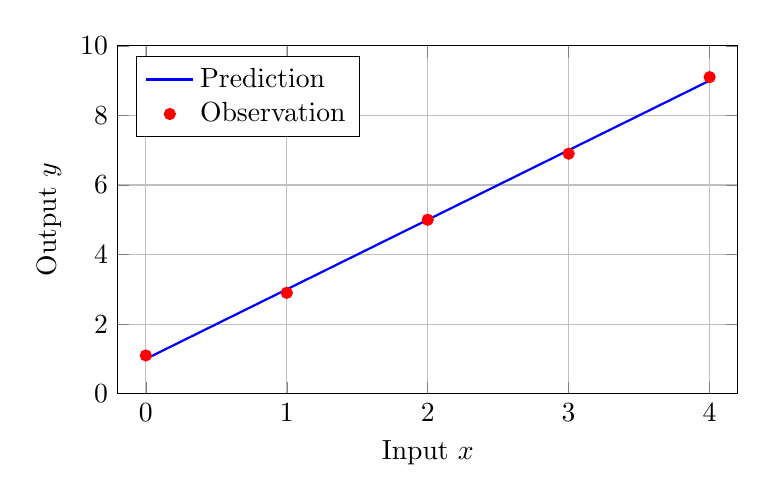
\begin{tikzpicture}
        \begin{axis}[
            width=0.78\textwidth,
            height=6cm,
            xlabel={Input $x$},
            ylabel={Output $y$},
            xmin=-0.2, xmax=4.2,
            ymin=0, ymax=10,
            xtick={0,1,2,3,4},
            grid=major,
            legend pos=north west,
            legend cell align=left
        ]
            \addplot[blue, thick, mark=none] coordinates {
                (0,1) (1,3) (2,5) (3,7) (4,9)
            };
            \addlegendentry{Prediction}
            \addplot[red, only marks, mark=*, mark size=2pt] coordinates {
                (0,1.1) (1,2.9) (2,5.0) (3,6.9) (4,9.1)
            };
            \addlegendentry{Observation}
        \end{axis}
    \end{tikzpicture}
    \caption{示例模型的观测值与预测结果}
    \label{fig:sample-results}
    \floatnote{资料来源：依据表\ref{tab:sample-results}中的示例数据绘制。}
\end{figure}

\subsubsection{误差分析}

将表\ref{tab:sample-results}中的数值代入式\eqref{eq:sample-rmse}，
可得 $E_{\mathrm{RMSE}}=\sqrt{0.008}\approx 0.0894$。
根据式\eqref{eq:sample-criterion}，有 $q(E_{\mathrm{RMSE}})=1$。
图表、公式和正文应采用一致的数据，正式写作时还应补充实验条件及误差来源分析。

\xmusection{算法排版示例}{Algorithm Typesetting}

以下伪代码使用模板已加载的算法环境，展示输入、输出、循环及条件语句的写法。
算法\ref{alg:sample-evaluation}对应前述误差计算和阈值判定过程。

\begin{algorithm}[htbp]
    \caption{示例模型的误差评价流程}
    \label{alg:sample-evaluation}
    \KwIn{观测值 $y_i$、预测值 $\hat{y}_i$、样本数量 $N$、阈值 $\tau$}
    \KwOut{均方根误差 $E_{\mathrm{RMSE}}$ 与判定结果 $q$}
    $S \leftarrow 0$\;
    \For{$i \leftarrow 1$ \KwTo $N$}{
        $S \leftarrow S + (y_i-\hat{y}_i)^2$\;
    }
    $E_{\mathrm{RMSE}} \leftarrow \sqrt{S/N}$\;
    \eIf{$E_{\mathrm{RMSE}} \leq \tau$}{
        $q \leftarrow 1$\;
    }{
        $q \leftarrow 0$\;
    }
\end{algorithm}

\xmusection{本章小结}{Chapter Summary}

本章通过示例数据展示了方法描述、公式推导、分段函数、结果表格、曲线图和算法。
结合第\ref{chap:sample-background}章，可观察同章与跨章引用的效果，
以及图、表和公式随章节自动编号的效果。


% ==================== 参考文献 ====================
% 参考文献：从 references.bib 文献数据库中生成参考文献列表。
\begin{reference}
\bibliography{references}
\end{reference}

% ==================== 附录 ====================
% 附录：在此环境内放置补充推导、数据、程序等内容。
\begin{appendix}
示例附录。
\end{appendix}

% ==================== 致谢 ====================
% 致谢：在此环境内填写对导师、合作者及资助方等的感谢。
\begin{acknowledgement}
示例致谢。
\end{acknowledgement}

% ==================== 答辩委员会名单页 ====================
% 插入位置由学院要求确定。
% 根据上方填写的主席和委员信息生成答辩委员会名单页。
\makecommittee

% ==================== 文档结束 ====================
% 文档结束。
\end{document}